\section{Analysis}

Section~\ref{sec:low-resource-nonen}에서 우리는 특정 언어 쌍(예: Lao--Thai, Basque--Korean)이 영어 skeleton을 활용한 추론보다 우수한 성능을 보일 수 있음을 확인하였다. 그러나 이러한 정량적 결과만으로는 해당 성능 향상의 원인을 특정하기 어렵다. 즉, 이러한 이득이 스켈레톤 자체의 생성 품질이 우수했기 때문인지, 아니면 타겟 언어와의 구조적 정렬에서 비롯된 시너지 효과인지는 여전히 불분명하다.

본 섹션에서는 이 두 요인을 분리하여 분석하기 위해, LLM-as-a-Judge를 활용한 criterion-based evaluation을 수행한다. 구체적으로, 우리는 생성된 스켈레톤의 Completeness(완결성), Specificity(구체성), Coherence(일관성)를 독립적으로 측정하여, 스켈레톤의 품질과 실제 추론 성능 간의 상관관계를 분석한다. 평가 방식의 세부 사항은 Appendix~\ref{}에서 확인할 수 있다.

\begin{figure}[!t]    
    \centering
    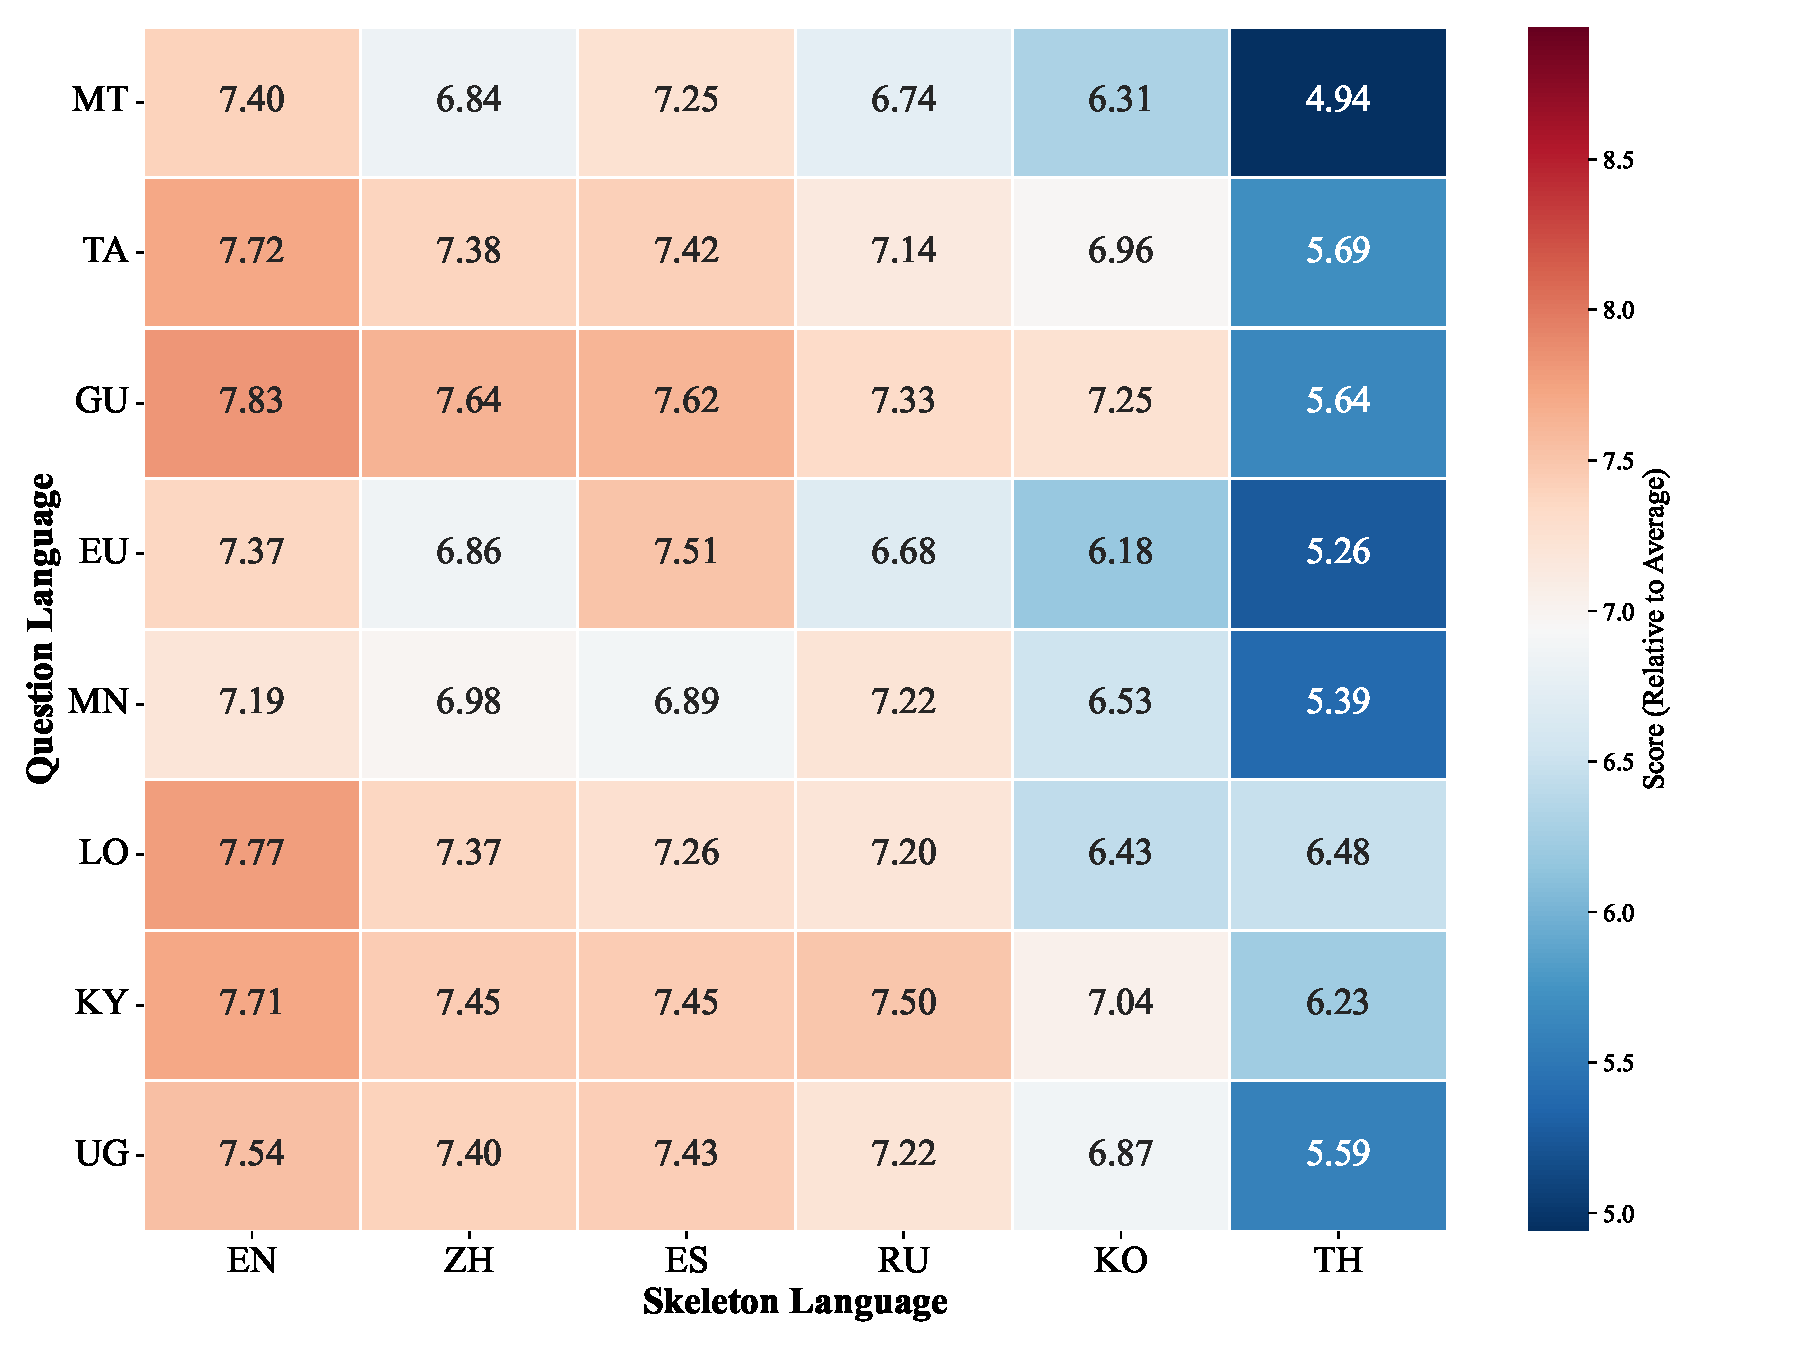
\includegraphics[width=\columnwidth]{Figures/Images/lang_pair_heatmap_styled.pdf}
    % 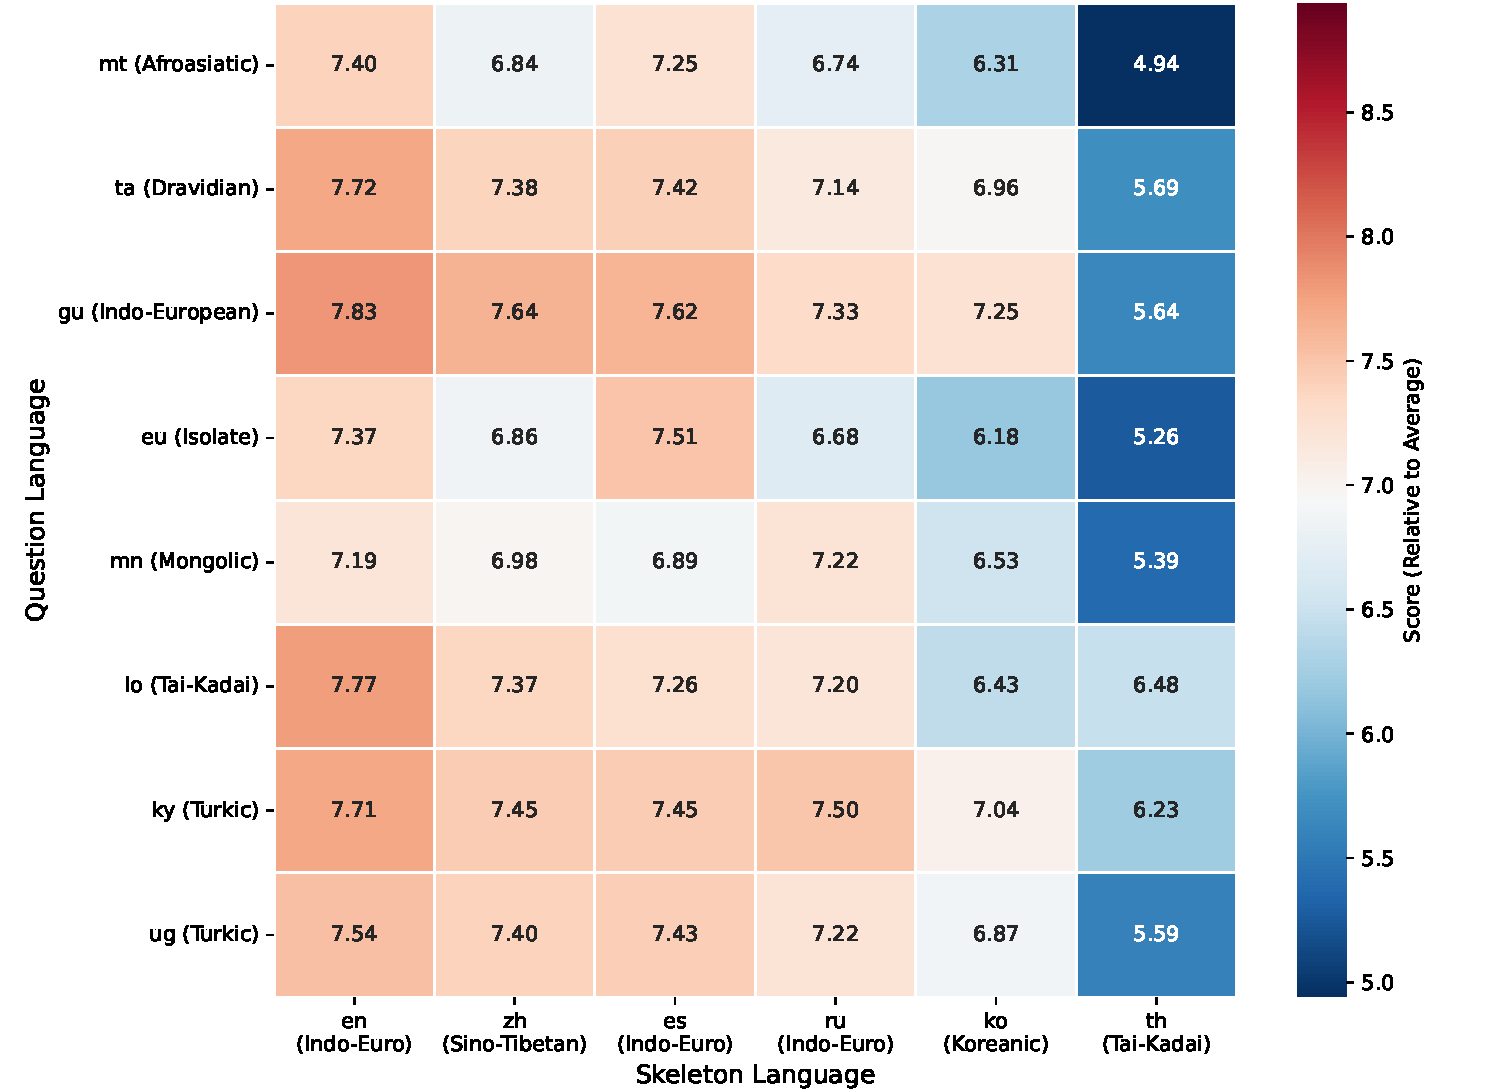
\includegraphics[width=\columnwidth]{Figures/Images/lang_pair_heatmap_cropped.pdf}
    \caption{\small Skeleton quality heatmap across language pairs. English skeletons yield highest quality (7.57), while Thai performs worst (5.65).}
    
\label{fig:lang_pair_heatmap}
    \vspace{-0.15in}
\end{figure}
Section~\ref{sec:low-resource-nonen}에서 관찰된 특정 언어 쌍의 성능 향상이 스켈레톤의 `생성 품질(Generation Quality)'에 기인한 것인지, 혹은 `구조적 정렬(Structural Alignment)' 덕분인지 규명하기 위해 정성적 평가를 수행하였다.

% \paragraph{Dominance of English Quality.}
% Figure~\ref{fig:lang_pair_heatmap}에 나타난 바와 같이, 전반적인 스켈레톤 품질은 English (Avg. 7.57)가 가장 높았으며, Spanish (7.35), Chinese (7.24), Russian (7.13)이 그 뒤를 이었다. 반면 Korean (6.69)과 Thai (5.65)는 상대적으로 낮은 점수를 기록하였다. 이러한 품질 순위는 영어가 가장 안정적인 anchor로 기능한 실험 결과와 일치한다.

\paragraph{Dominance of English Quality.} 
Figure~\ref{fig:lang_pair_heatmap}에 나타난 바와 같이, 언어별 스켈레톤의 본질적 품질은 English (Avg. 7.57)가 가장 높았으며, Spanish (7.35), Chinese (7.24), Russian (7.13)이 그 뒤를 이었다. 반면 Korean (6.69)과 Thai (5.65)는 상대적으로 낮은 점수를 기록하였다. 이는 사전학습 데이터의 양이 풍부한 영어가 스켈레톤 생성 능력면에서 가장 안정적인 앵커임을 보여주며, 앞선 실험(Section~\ref{sec:low-resource-nonen}에서 영어가 전반적으로 높은 성능을 보인 이유를 뒷받침한다.

\paragraph{Quality-Performance Inversion.} 
그러나 흥미로운 점은 스켈레톤의 품질 점수와 실제 추론 성능 간의 역전 현상(Inversion)이다. \textsc{Lao~(lo)}의 경우, \textsc{Thai~(th)} 스켈레톤의 품질(6.48)은 영어(7.77)보다 1.29점이나 낮았음에도, 실제 추론 성능은 태국어 스켈레톤이 +2.81점 높았다. 유사하게 \textsc{Basque~(eu)}에서도 \textsc{Korean~(ko)} 스켈레톤(6.18)은 영어(7.37)보다 품질이 1.19점 떨어졌으나, 성능은 오히려 +6.32점 높게 나타났다. 반면, 언어적 정렬이 부재한 경우에는 이러한 역전이 발생하지 않았다. \textsc{Uyghur~(ug)}에서 중국어 스켈레톤의 품질(7.40)은 영어(7.54)와 거의 동등하였으나 성능은 −6.45점 하락하였고, \textsc{Mongolian~(mn)}에서도 러시아어 스켈레톤(7.22)이 영어(7.19)보다 소폭 높은 품질을 보였음에도 성능은 −5.53점 감소하였다. 이러한 결과는 Linguistic Alignment(언어적 정렬)가 스켈레톤의 품질의 열세를 상쇄할 수 있음을 시사한다.
% \paragraph{Quality-Performance Inversion.}
% 그러나 흥미로운 점은 스켈레톤의 품질 점수와 실제 추론 성능 간의 역전 현상(Inversion)이다. \textsc{Lao (lo)}의 경우, \textsc{Thai (th)} 스켈레톤의 품질 점수(6.48)는 영어(7.77)보다 1.29점 낮았음에도, 실제 추론 성능은 태국어 스켈레톤이 +2.81점 높았다. 유사하게 \textsc{Basque (eu)}에서도 \textsc{Korean (ko)} 스켈레톤(6.18)은 영어(7.37)보다 품질이 1.19점 떨어졌으나, 성능은 오히려 +6.32점 높게 나타났다. 반면, 언어적 정렬이 부재한 경우에는 이러한 역전이 발생하지 않았다. \textsc{Uyghur (ug)}에서 중국어 스켈레톤의 품질(7.40)은 영어(7.54)와 거의 동등하였으나 성능은 −6.45점 하락하였고, \textsc{Mongolian (mn)}에서도 러시아어 스켈레톤(7.22)이 영어(7.19)보다 소폭 높은 품질을 보였음에도 성능은 −5.53점 감소하였다. 이러한 결과는 Linguistic Alignment(언어적 정렬)가 스켈레톤의 품질의 열세를 상쇄할 수 있음을 시사한다. 

\paragraph{Implication}
이러한 Quality--Performance Mismatch 현상은 \LASEF의 당위성을 강력하게 뒷받침한다. 만약 추론 성능이 단순히 스켈레톤의 생성 품질에 비례한다면, 가장 완성도 높은 영어가 언제나 최적해(optimal solution)였을 것이다. 그러나 본 분석은 본질적 품질이 다소 낮더라도 타겟 언어와 구조적으로 정렬될 경우, 고품질의 영어 스켈레톤을 능가할 수 있음을 입증한다. 더욱이 이러한 `숨겨진 정렬(hidden alignment)'은 표면적인 품질이나 단순한 언어학적 분류만으로는 사전에 예측하기 어렵다. 따라서 스켈레톤 언어를 고정된 요소로 간주하기보다 언어의 조합을 exploration해야 함을 시사한다.

% 이는 스켈레톤 언어를 고정된 상수로 취급하는 대신, \LASEF를 통해 데이터에 내재된 최적의 언어 조합을 체계적으로 탐색해야 함을 시사한다.
% 이러한 `Quality-Performance Mismatch' 현상은 본 논문이 제안하는 \LASEF의 당위성을 뒷받침한다. 만약 스켈레톤의 성능이 텍스트 품질에 비례한다면, 단순히 가장 잘 쓰인(well-written) 영어 스켈레톤을 사용하는 것이 최적해일 것이다. 그러나 위 분석 결과는 낮은 품질의 스켈레톤이라도 ``타겟 언어와 구조적으로 잘 정렬되어 있으면, 높은 품질의 영어 스켈레톤을 능가할 수 있음''을 증명한다. 중요한 점은, 이러한 '숨겨진 정렬(hidden alignment)'은 겉보기 품질이나 단순한 언어학적 분류만으로는 사전에 예측하기 어렵다는 것이다. 따라서 고정된 언어를 사용하는 대신, \LASEF와 같이 다양한 언어 조합을 경험적으로 탐색하고 최적의 스켈레톤 언어를 찾아내는 체계적인 접근이 필수적으로 요구된다.